\section{Method}
\label{sec:method}
We present TopoPRM, a framework comprising three components: (1)~a multi-source reward module that extracts dependency DAGs from reasoning traces and computes deterministic topology and continuity rewards; (2)~a post-training pipeline that uses these rewards within a standard SFT-then-GRPO stack to produce a teacher with structured reasoning capability; and (3)~a reverse-KL distillation stage that compresses the teacher into a smaller, more efficient student.
Figure~\ref{fig:overview} illustrates the overall architecture.

\subsection{Problem Setup}

Given an input $x=(q,s)$, where $q$ is a mathematical problem and $s$ is optional context, a policy $\pi_\theta$ generates a completion $y \sim \pi_\theta(\cdot\mid x)$.
Outcome-only RLVR uses a sparse correctness signal $r_{\mathrm{out}}(x,y)\in\{0,1\}$, which is effective for final-answer accuracy but insufficient for controlling intermediate reasoning structure.
Our goal is to add deterministic process supervision without introducing learned reward models or human step-level annotations.

\begin{figure}[t]
    \centering
    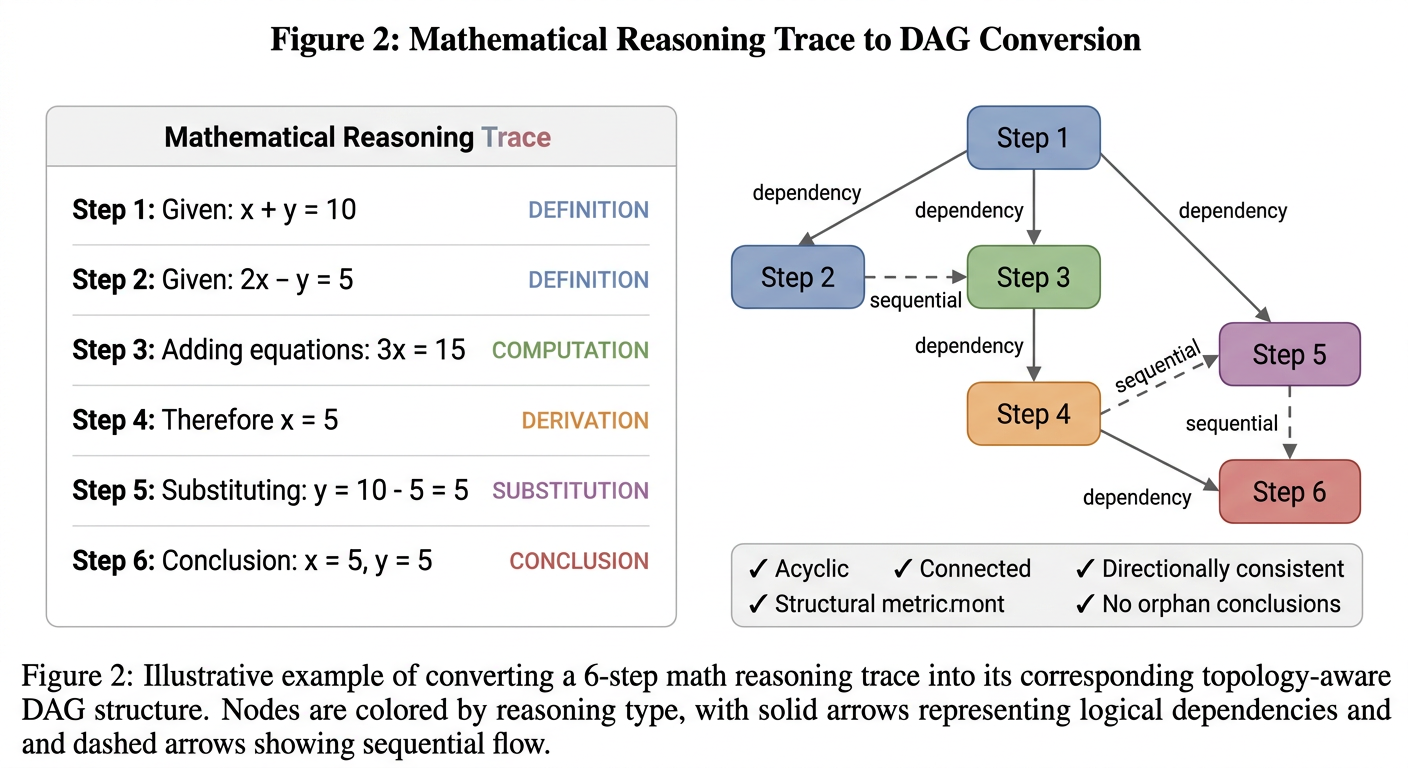
\includegraphics[width=0.98\linewidth]{figures/Fig2.DAG_Visualization.png}
    \caption{Transformation of a free-form reasoning trace into a
    verifiable dependency DAG. Step types are inferred by rule-based
    classification; virtual edges are built from expression/claim reuse,
    while solid and double-barrier edges provide weak/no-reward structure.}
    \label{fig:dag_extraction}
\end{figure}

\subsection{Topology-Aware Reward Fusion}
\label{sec:reward_module}

\subsubsection{Trace-to-DAG Extraction}
For reasoning traces $y=(s_1,\ldots,s_T)$ in the \texttt{<think>} block, we apply a deterministic extractor:
\begin{equation}
\label{eq:extractor}
\mathcal{G}=\mathcal{E}(y)=(\mathcal{V},\mathcal{A}),
\end{equation}
where each node $v_i\in\mathcal{V}$ corresponds to reasoning step $s_i$, and each directed edge $(u,v)\in\mathcal{A}$ indicates a rule-defined dependency (expression reuse, claim reference, or structural connector).
The extractor segments the trace by numbered steps, mathematical delimiters, and logical connectives, then detects dependencies through shared mathematical expressions and variable references.
To reduce parser artifacts, claim extraction is sentence-level rather than phrase-level:
heading fragments and unfinished prefixes (e.g., ``all cases are:'' without a predicate) are filtered out before graph construction.
This prevents malformed claim nodes from dominating dependency matching.

Node-level verdicts use a hybrid policy.
If reference DAG verdicts are available, they are copied directly.
Otherwise, we apply deterministic fallback rules based on support evidence, conclusion support status, and explicit contradiction markers to assign \texttt{correct}/\texttt{incorrect}/\texttt{unverifiable}.
This avoids the degenerate all-\texttt{unverifiable} regime during diagnostics.

% See Appendix for detailed scope-of-verifiability discussion.
% We emphasise an important scope distinction: the extracted graph is an inferred dependency DAG induced by deterministic rules, not a ground-truth proof graph.
% Deterministic extraction ensures reproducible reward computation, not semantic completeness of dependency recovery.

\subsubsection{Topology Reward}
The topology reward captures global structural regularity of the extracted DAG:
\begin{equation}
\label{eq:r_topo}
r_{\mathrm{topo}}(\mathcal{G}) =
\lambda_b\,\mathbb{1}[|\mathcal{V}|>0]
+\lambda_a\,\mathbb{1}[\mathcal{G}\ \text{acyclic}]
+\lambda_o\,\mathbb{1}[\rho_{\mathrm{orphan}}(\mathcal{G})=0]
+\lambda_d\,\delta(\mathcal{G})
+\lambda_k\,\kappa(\mathcal{G},\mathcal{G}^{*}),
\end{equation}
where $\rho_{\mathrm{orphan}}$ is the fraction of unsupported conclusion nodes, $\delta$ is dependency-direction consistency, and $\kappa$ is optional reference-edge coverage against a weak reference graph $\mathcal{G}^{*}$.
A hard gate sets the score to zero when the extracted graph is invalid.
When no reference graph is available, the $\kappa$ term is disabled and the score is normalized by the remaining active coefficients.
For auditability, we log raw indicators ($\rho_{\mathrm{orphan}},\delta,\kappa$), per-term contributions
($\lambda_b\mathbb{1}[|\mathcal{V}|>0]$, $\lambda_a\mathbb{1}[\mathrm{acyclic}]$, $\lambda_o\mathbb{1}[\rho_{\mathrm{orphan}}=0]$, $\lambda_d\delta$, $\lambda_k\kappa$),
and the final normalized $r_{\mathrm{topo}}$ for each sample.

\subsubsection{Continuity Reward}
The continuity reward captures local support traceability across reasoning steps:
\begin{equation}
\label{eq:r_cont}
r_{\mathrm{cont}}(y)=
\begin{cases}
1.0, & \eta(y)=1,\\
0.8\,\eta(y), & \eta(y)<1,
\end{cases}
\qquad
\eta(y)=\frac{1}{T}\sum_{i=1}^{T}\mathbb{1}[\mathrm{supported}(s_i,s_{<i},q)].
\end{equation}
A step is marked as supported if it reuses prior claims or expressions, or explicitly cites problem givens, based on deterministic regex-based matching.
Full coverage ($\eta{=}1$) yields the maximum reward; partial coverage is discounted by a factor of $0.8$.

%\subsubsection{Scope of Verifiability}
% See Appendix for extended discussion on reward aggregation strategies.
% Our use of ``verifiable'' is operational: once a trace is produced, all reward values are computed by deterministic procedures and are therefore reproducible and auditable.
% This is distinct from semantic proof verification; we do not claim step-correctness guarantees or logical completeness.

\subsection{Post-Training and Optimisation}
\label{sec:post_training}
The post-training pipeline consists of two stages: SFT cold-start followed by GRPO with the TopoPRM reward module.

\begin{figure*}[t]
    \centering
    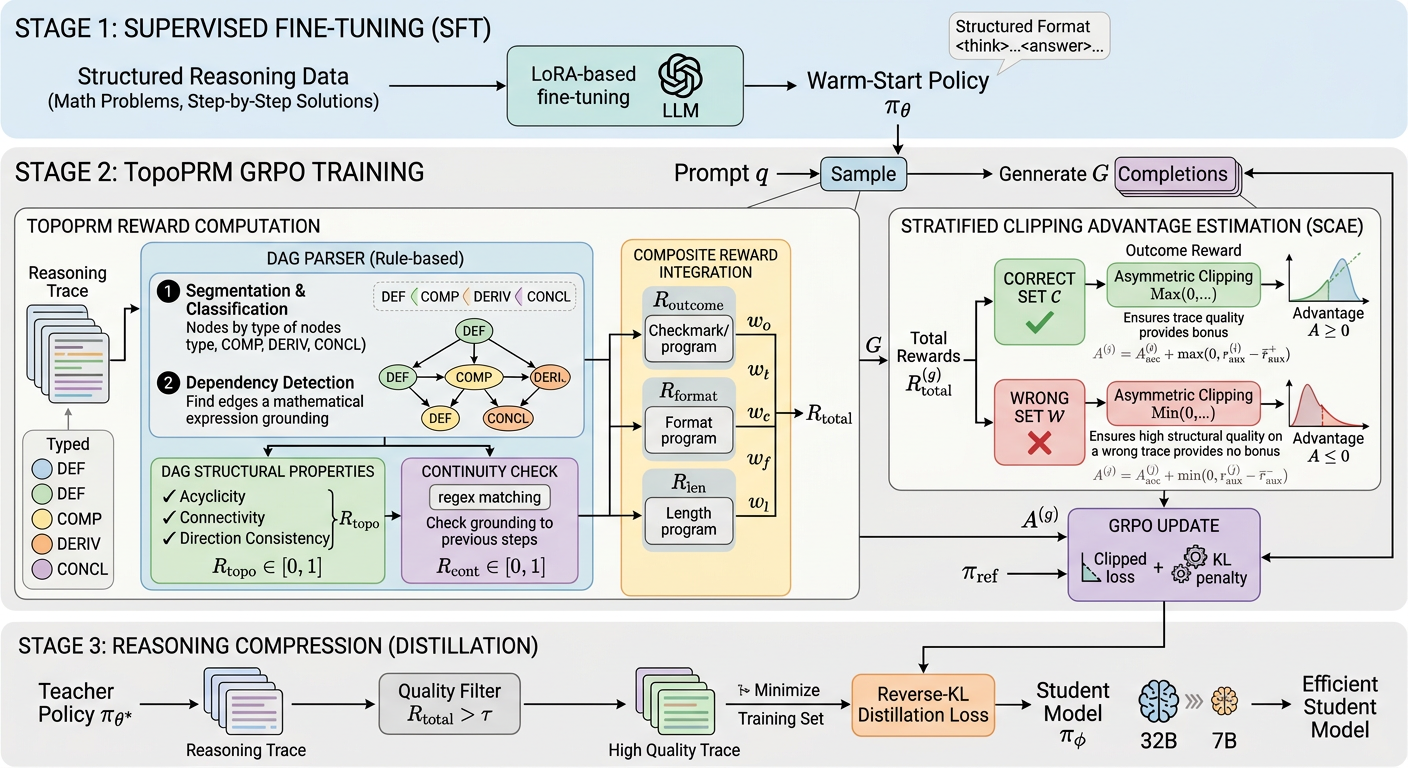
\includegraphics[width=0.98\linewidth]{figures/Ai_Framework.png}
    \caption{Overview of TopoPRM. The reward module extracts dependency DAGs from reasoning traces and computes deterministic process rewards. Stage~I trains a teacher via SFT cold-start followed by GRPO with hierarchical reward aggregation. Stage~II applies process-aware filtering and reverse-KL distillation to obtain a compact student.}
    \label{fig:overview}
\end{figure*}

\subsubsection{Stage~I: SFT Cold-Start}

We fine-tune the base model on a mixture of Chinese mathematical critique examples and English math reasoning problems to establish basic format compliance and reasoning capability.
This produces a checkpoint $\pi_\theta$ that serves as the initialisation for reinforcement learning.

\subsubsection{Stage~II: GRPO with Hierarchical Reward Aggregation}

Each training step samples completions from $\pi_\theta$, extracts dependency DAGs, and computes five reward signals: outcome correctness $r_{\mathrm{out}}$, topology $r_{\mathrm{topo}}$, continuity $r_{\mathrm{cont}}$, format compliance $r_{\mathrm{fmt}}$, and length penalty $r_{\mathrm{len}}$.

\paragraph{Hierarchical aggregation.}
A naive weighted sum can mis-rank traces when high process scores compensate for incorrect answers, and in practice causes reward collapse when batch-level reward variance approaches zero.
We instead adopt a hierarchical formulation that separates base correctness from process-level gain:
\begin{equation}
\label{eq:r_base}
r_{\mathrm{base}} = w_o \cdot r_{\mathrm{out}} + w_f \cdot r_{\mathrm{fmt}} + w_l \cdot r_{\mathrm{len}},
\end{equation}
\begin{equation}
\label{eq:r_total}
r_{\mathrm{total}} = r_{\mathrm{base}} \cdot \bigl(1 + \alpha \cdot \tilde{r}_{\mathrm{topo}} + (1-\alpha) \cdot \tilde{r}_{\mathrm{cont}}\bigr),
\end{equation}
where $\tilde{r}_{\mathrm{topo}}$ and $\tilde{r}_{\mathrm{cont}}$ are batch-level min-max rescaled to $[0,1]$, and $\alpha$ controls the topology-continuity balance.
Process rewards act as a multiplicative gain on the base signal rather than an additive offset, preserving answer-correctness primacy while amplifying structural quality differences.

\paragraph{Anti-collapse mechanisms.}
To prevent reward collapse during GRPO training, we use three complementary mechanisms:
(i)~batch-level min-max rescaling ensures that process reward components retain sufficient spread;
(ii)~reward temperature scaling ($\tau{=}2.0$) amplifies small differences via $r \leftarrow \mu + (r - \mu) \cdot \tau$;
(iii)~a minimum-variance guard injects small Gaussian noise ($\epsilon{=}0.01$) when the batch reward standard deviation falls below a threshold ($\sigma_{\min}{=}0.005$).

\paragraph{Correctness-first stratification.}
As an additional safeguard, we partition each batch into correct and incorrect strata:
\begin{equation}
\label{eq:scae_partition}
\mathcal{C}=\{i\mid r_{\mathrm{out}}^{(i)}\ge\tau\},
\qquad
\mathcal{W}=\{i\mid r_{\mathrm{out}}^{(i)}<\tau\}.
\end{equation}
Within each stratum, rewards are standardised and asymmetrically clipped:
\begin{equation}
\label{eq:scae_shape}
\tilde{r}^{(i)}=
\begin{cases}
\mathrm{clip}(z^{(i)},0,1.5), & i\in\mathcal{C},\\
\mathrm{clip}(z^{(i)},-1.5,0), & i\in\mathcal{W},
\end{cases}
\end{equation}
guaranteeing that answer-correct traces remain non-negative and answer-incorrect traces remain non-positive after shaping.

\subsection{Distillation and Reasoning Compression}
\label{sec:compression}

Let $\pi_T$ denote the teacher after Stage~II and $\pi_S$ the student to be trained.
We first construct a filtered dataset $\mathcal{D}_f$ by retaining only teacher traces whose composite reward exceeds a quality threshold ($R_{\mathrm{total}} > 0.7$).
Distillation minimises the reverse KL divergence:
\begin{equation}
\label{eq:distill}
\mathcal{L}_{\mathrm{RKL}}=
\mathbb{E}_{x\sim\mathcal{D}}\left[
D_{\mathrm{KL}}\!\left(\pi_S(\cdot\mid x)\,\|\,\pi_T(\cdot\mid x)\right)
\right].
\end{equation}
Reverse KL is mode-seeking: it encourages $\pi_S$ to concentrate on high-probability teacher modes rather than averaging over diverse outputs~\citep{sang2026opsdc}.
In our setting, this compresses graph-enriched teacher reasoning into compact chain-like student reasoning without requiring the student to produce explicit DAG output.

The distillation stage also incorporates length-aware reward shaping during data selection: correct answers receive higher weight as reasoning length decreases (rewarding conciseness), incorrect answers are penalised more heavily as length increases (discouraging verbose but wrong reasoning), and traces exceeding a maximum length threshold are excluded entirely.
These criteria ensure that the student inherits both structural quality and reasoning efficiency from the teacher.

From an RLVR perspective, this design follows a simple separation
principle. The training \emph{direction} is determined in Stage~II by
verifiable task/process rewards (outcome, topology, continuity, format),
while Stage~III distillation primarily improves \emph{token-level
efficiency} by concentrating student probability mass on high-quality
teacher modes. This keeps the optimisation target anchored to
deterministic verifiable signals, while still benefiting from dense
token-level compression in the final student model.

\begin{algorithm}[t]
\caption{TopoPRM Training Pipeline}
\label{alg:topoprm}
\begin{algorithmic}[1]
\Require Base model $\pi_0$, SFT data $\mathcal{D}_{\mathrm{sft}}$, RL prompts $\mathcal{D}_{\mathrm{rl}}$
\Ensure Teacher $\pi_T$ and optional student $\pi_S$
\State $\pi_\theta \leftarrow \mathrm{SFT}(\pi_0,\mathcal{D}_{\mathrm{sft}})$ \Comment{Cold-start}
\For{each GRPO batch on $\mathcal{D}_{\mathrm{rl}}$}
  \State Sample completions; extract dependency DAGs via $\mathcal{E}$
  \State Compute $r_{\mathrm{out}},r_{\mathrm{topo}},r_{\mathrm{cont}},r_{\mathrm{fmt}},r_{\mathrm{len}}$
  \State Aggregate via Eq.~\ref{eq:r_total}; shape via Eq.~\ref{eq:scae_shape}
  \State Update $\pi_\theta$ using GRPO with shaped rewards
\EndFor
\State $\pi_T \leftarrow \pi_\theta$ \Comment{Teacher ready}
\If{distillation enabled}
  \State Filter teacher traces by process-aware criteria $\to \mathcal{D}_f$
  \State Train $\pi_S$ by minimising $\mathcal{L}_{\mathrm{RKL}}$ (Eq.~\ref{eq:distill})
\EndIf
\end{algorithmic}
\end{algorithm}

